\section{Vista de Escenarios}
En la siguiente figura, la \ref{fig:Diagrama de Casos de Uso - Vista de Escenarios}, se muestra la vista de escenarios representada por un diagrama de casos de uso. Este diagrama refleja los requerimientos funcionales principales del sistema. Cada caso de uso lo hemos identificado un una nomenclatura CU'X', siendo la letra 'X' el número del caso de uso al que se hace referencia.
\\
\begin{figure}[!h]
	\centering
	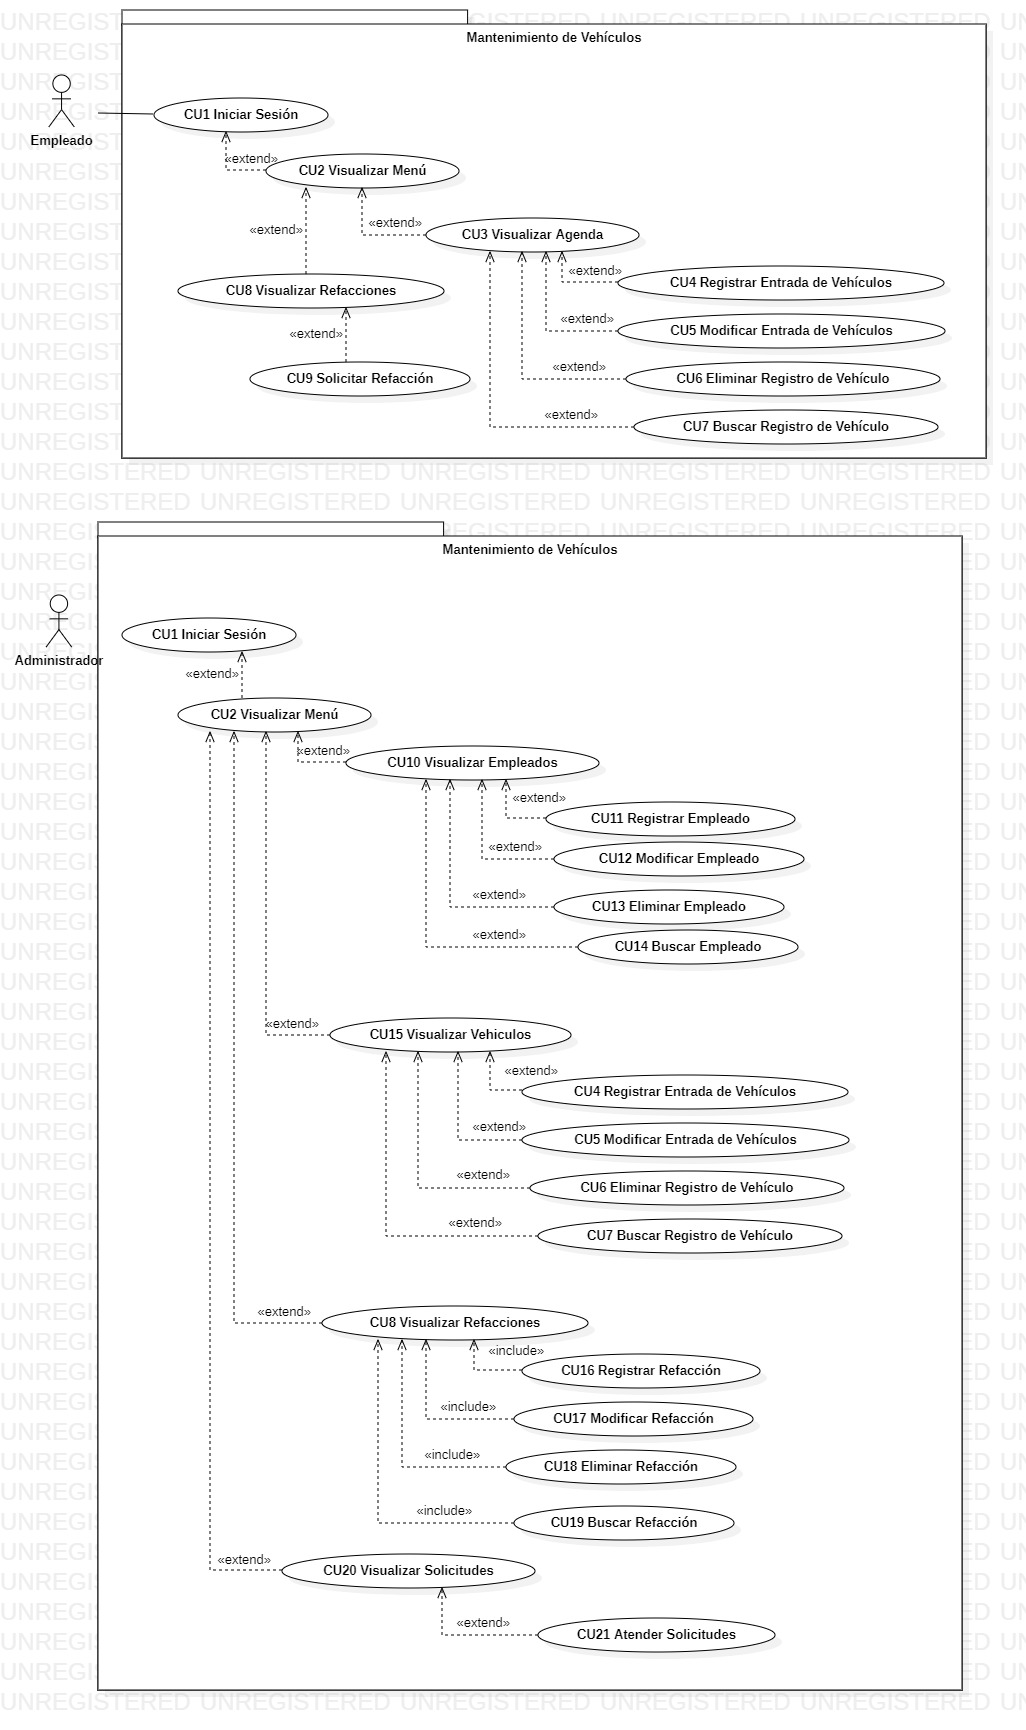
\includegraphics[width=1\textwidth]{./diseno/vescenarios/imagenes/vistaEscenarios}
	\caption{Diagrama de Casos de Uso - Vista de Escenarios}
	\label{fig:Diagrama de Casos de Uso - Vista de Escenarios}
\end{figure}
\\
A continuación se describen a detalle cada uno de los casos de uso que serán implementados en el sistema. Cada uno de estos casos también llevará un diseño de la UI (Interfaz de Usuario) para poder explicar el procedimiento de cada uno de los procesos. Cabe mencionar que estos casos de uso van de la mano con las historias de usuario descritas en el capítulo \ref{chap: historias de usuario}. 

\clearpage

%Contenido de la vista de escenarios
\subsection{CU1 Iniciar Sesión}
Esta pantalla (figura \ref{fig:Pantalla Iniciar Sesion - Vista de Escenarios}) será la primera en aparecer al ejecutarse el sistema. Se compone de un pequeño formulario donde el usuario (Mecánico) deberá teclear sus credenciales otorgadas por la administración de la empresa. Una vez ingresados de manera correcta, deberá pulsar el botón 'Ingresar'.
\\
En caso de que el usuario desee salir del sistema, solo deberá pulsar el botón 'Salir'. 
\\

\begin{figure}[!h]
	\centering
	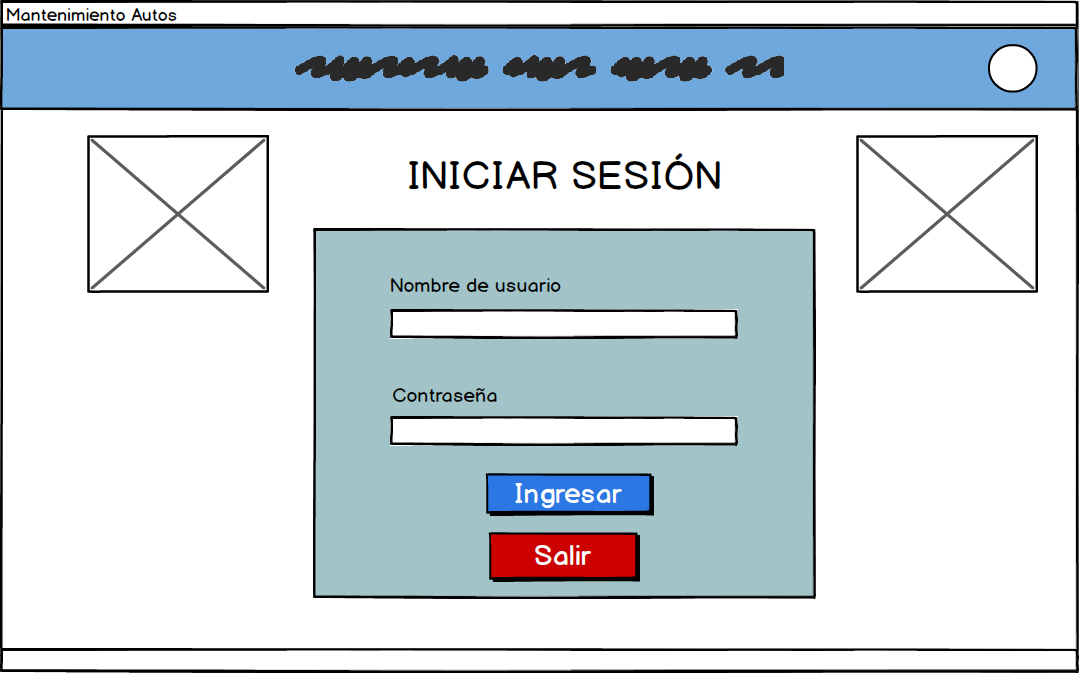
\includegraphics[width=1\textwidth]{./diseno/vescenarios/imagenes/Login}
	\caption{Pantalla Iniciar Sesión - Vista de Escenarios}
	\label{fig:Pantalla Iniciar Sesion - Vista de Escenarios}
\end{figure}
En ese sentido, si el usuario ingresa erróneamente sus credenciales de autenticación, el sistema mostrará un mensaje de alerta (\ref{fig:Alerta1 - Vista de Escenarios}).
\\
\begin{figure}[!h]
	\centering
	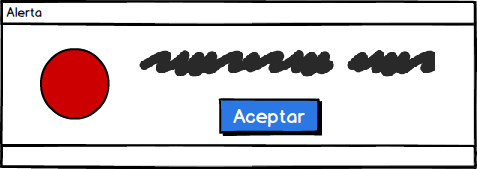
\includegraphics[width=0.5\textwidth]{./diseno/vescenarios/imagenes/alerta}
	\caption{Alerta Datos Erróneos - Vista de Escenarios}
	\label{fig:Alerta1 - Vista de Escenarios}
\end{figure}
\clearpage
\subsection{CU2 Visualizar Menú}
Al momento de ingresar las credenciales y que el sistema otorgue acceso al usuario, aparecerá una pantalla muy simular a la que mostramos a continuación (figura \ref{fig:Pantalla Visualizar Menu - Vista de Escenarios}). Esta pantalla posee el mismo diseño que el inicio de sesión (figura \ref{fig:Pantalla Iniciar Sesion - Vista de Escenarios}), solo que esta vez, se muestran tres opciones principales. 
\begin{itemize}
	\item \textbf{Gestionar Agenda:} En esta opción se desplegará otra pantalla que le dará acceso al usuario a toda la información que desee saber sobre los registros de los vehículos que estén dentro del taller además de la gestión de los mismos.
	\item \textbf{Gestionar Refacciones:} En dado caso que el usuario desee saber sobre la existencia de alguna refacción en particular dentro del almacén del taller además de generar una solicitud para la obtención de una si en necesario.
	\item \textbf{Cancelar:} El usuario desea salir de esa pantalla y regresar a la pantalla de Iniciar Sesión (figura \ref{fig:Pantalla Iniciar Sesion - Vista de Escenarios}).
\end{itemize}
\begin{figure}[!h]
	\centering
	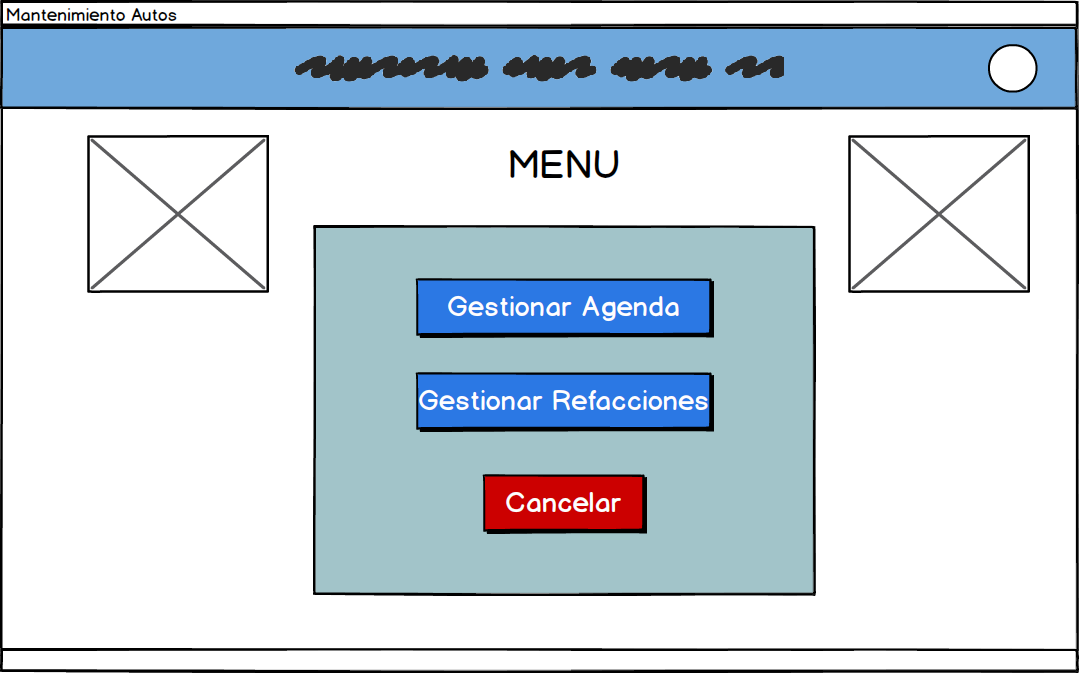
\includegraphics[width=1\textwidth]{./diseno/vescenarios/imagenes/VisualizarMenu}
	\caption{Pantalla Visualizar Menu - Vista de Escenarios}
	\label{fig:Pantalla Visualizar Menu - Vista de Escenarios}
\end{figure}
\clearpage
\subsection{CU3 Visualizar Agenda}
Supongamos que el usuario decide ver todos los registros de los vehículos dentro del taller y elige la opción de Gestionar Agenda, inmediatamente esta pantalla (figura \ref{fig:Pantalla Visualizar Agenda - Vista de Escenarios}) aparecerá. Compuesta principalmente por una tabla donde se mostrarán a manera de lista cada uno de los registros que estén almacenados en la base de datos, en caso de que no exista ningún registro, dicha tabla se mostrará vacía.
\\
En la parte superior derecha hay una barra de búsqueda, se explica a detalle este proceso mas adelante (véase \ref{sub:buscar registro}). 
\\
En la parte inferior se despliegan una serie de botones que permitirán al usuario gestionar esta tabla de registros que se le presentan:
\begin{itemize}
	\item \textbf{Actualizar Registro:} Permite al usuario actualizar la tabla una vez que este haya realizado algún cambio en los registros.
	\item \textbf{Registrar Vehículo:} Despliega una pantalla con un formulario de registro.
	\item \textbf{Modificar Vehículo:} Despliega una pantalla con un formulario de actualización.
	\item \textbf{Eliminar Vehículo:} Despliega una pantalla con un 'mensaje de seguridad'. 
	\item \textbf{Salir:} Regresar al menú de opciones (figura \ref{fig:Pantalla Visualizar Menu - Vista de Escenarios}). 
\end{itemize}
\begin{figure}[!h]
	\centering
	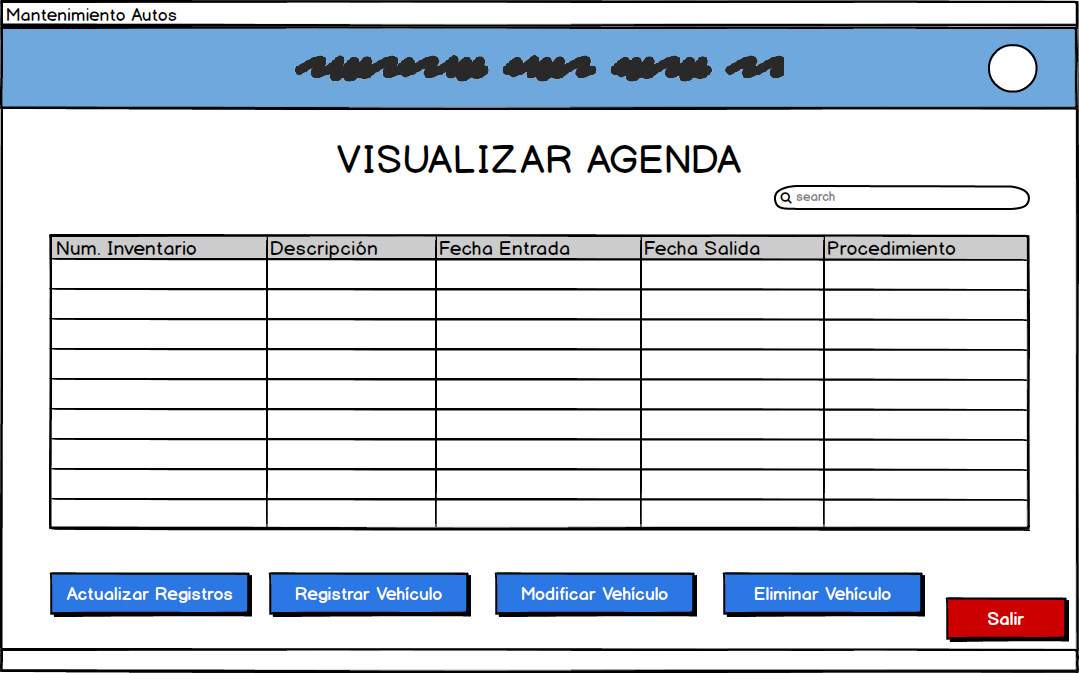
\includegraphics[width=1\textwidth]{./diseno/vescenarios/imagenes/VisualizarAgenda}
	\caption{Pantalla Visualizar Agenda - Vista de Escenarios}
	\label{fig:Pantalla Visualizar Agenda - Vista de Escenarios}
\end{figure}
Cabe señalar que el usuario debe de elegir un registro en la tabla para poder realizar alguna de las acciones antes mencionadas, de lo contrario aparecerá un 'mensaje de alerta' (figura \ref{fig:Alerta - Vista de Escenarios}) donde le de a entender al usuario lo que debe de hacer antes de relizar cualquier acción sobre algún registro.
\begin{figure}[!h]
	\centering
	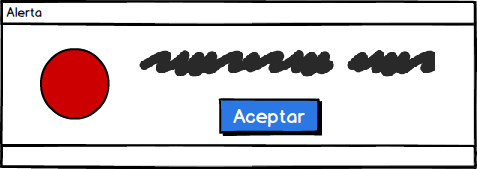
\includegraphics[width=0.5\textwidth]{./diseno/vescenarios/imagenes/alerta}
	\caption{Alerta Elección de Registro - Vista de Escenarios}
	\label{fig:Alerta - Vista de Escenarios}
\end{figure}
\clearpage
\subsection{CU4 Registrar Entrada de Vehículo}
Pantalla que aparece al presionar el botón de 'Registrar Vehículo' en la visualización de agenda (figura \ref{fig:Pantalla Visualizar Menu - Vista de Escenarios}). Este formulario le solicita al usuario los siguientes campos: Número de Inventario, Descripción, Fecha de Entrada, Fecha de Salida y el Procedimiento que se le hará al vehículo. 
\\
Cuenta con dos botones en la parte inferior, uno para proceder a enviar el registro a la base de datos y otro para cancelar en caso de que el usuario así lo desee. 
\\
\begin{figure}[!h]
	\centering
	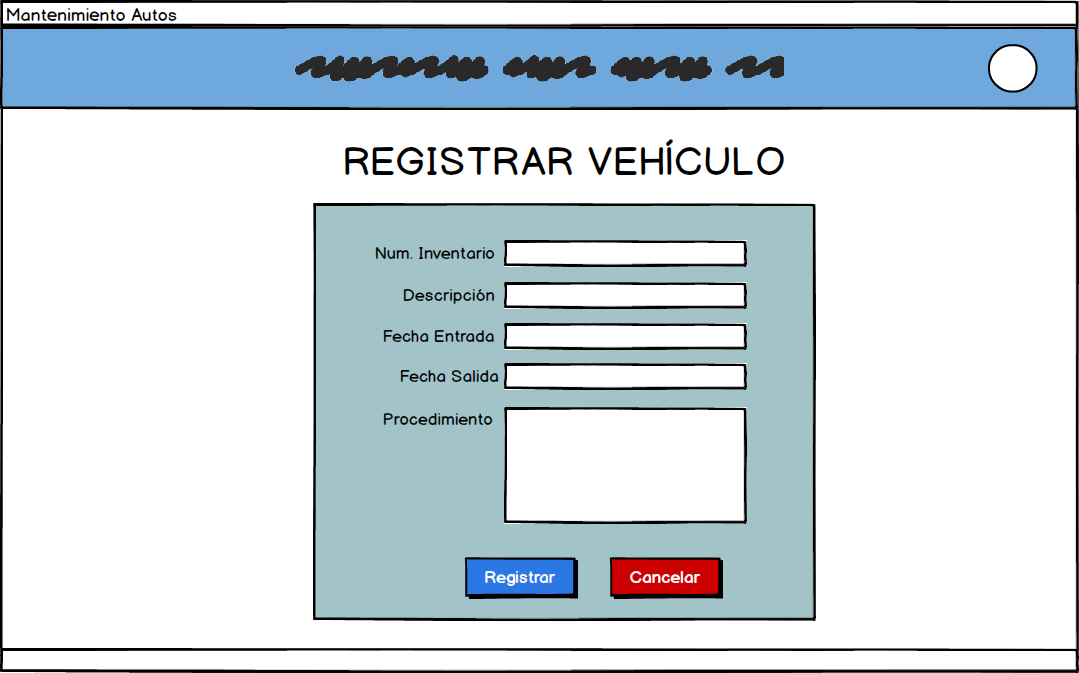
\includegraphics[width=0.9\textwidth]{./diseno/vescenarios/imagenes/registrarVehiculo}
	\caption{Pantalla Registrar Vehículo - Vista de Escenarios}
	\label{fig:Pantalla Registrar Vehículo - Vista de Escenarios}
\end{figure}
\\
En caso de que el usuario ingrese algún dato mal, es decir, que los campos no estén llenos o el formato de la información no es el correcto, aparecerá una alerta como la que se muestra a continuación (figura \ref{fig:Alerta2 - Vista de Escenarios}):
\begin{figure}[!h]
	\centering
	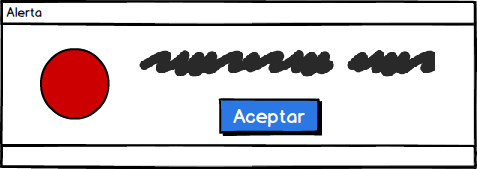
\includegraphics[width=0.4\textwidth]{./diseno/vescenarios/imagenes/alerta}
	\caption{Alerta Confirmación de Registro - Vista de Escenarios}
	\label{fig:Alerta2 - Vista de Escenarios}
\end{figure}
\clearpage
\subsection{CU5 Modificar Registro de Vehículo}
Esta pantalla es muy similar a la del 'Registro de Vehículo' (figura \ref{fig:Pantalla Registrar Vehículo - Vista de Escenarios}), solo que esta vez cuando el usuario desee modificar un registro en específico este formulario aparecerá con todos los campos llenos para que el usuario pueda modificar el que necesite. 
\\
En la parte inferior de la pantalla hay dos botones; el primero de ellos, el botón 'Modificar' lleva la información a la base de datos. El segundo, botón 'Cancelar' cierra esta pantalla y no hay alteración en los datos. 
\begin{figure}[!h]
	\centering
	\includegraphics[width=1\textwidth]{./diseno/vescenarios/imagenes/modificarVehículo}
	\caption{Pantalla Modificar Registro de Vehículo - Vista de Escenarios}
	\label{fig:Pantalla Modificar Registro de Vehículo - Vista de Escenarios}
\end{figure}
\\
En caso de que el usuario actualice algún dato mal, es decir, que los campos no estén llenos o el formato de la información no es el correcto, aparecerá una alerta como la que se muestra a continuación (figura \ref{fig:Alerta3 - Vista de Escenarios}):
\begin{figure}[!h]
	\centering
	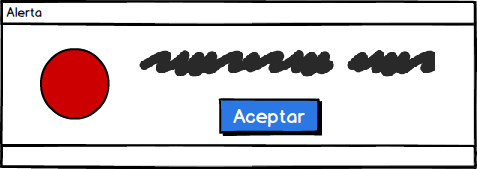
\includegraphics[width=0.5\textwidth]{./diseno/vescenarios/imagenes/alerta}
	\caption{Alerta Modificación - Vista de Escenarios}
	\label{fig:Alerta3 - Vista de Escenarios}
\end{figure}
\clearpage
\subsection{CU6 Eliminar Registro de Vehículo}
Esta pantalla es muy similar a la de Registrar Vehículo (figura \ref{fig:Pantalla Registrar Vehículo - Vista de Escenarios}) y a la de Modificar Vehículo (figura \ref{fig:Pantalla Modificar Registro de Vehículo - Vista de Escenarios}), sin embargo, esta pantalla esta diseñada para ser un 'mensaje de seguridad'. Muestra los datos que el usuario desea eliminar y al pulsar el botón 'Aceptar', el sistema ordena a la base de datos eliminar ese registro. Por otro lado, el botón 'Cancelar', cierra ese mensaje de seguridad y volvemos a la pantalla de Visualizar Agenda (figura \ref{fig:Pantalla Visualizar Agenda - Vista de Escenarios}).
\\
\begin{figure}[!h]
	\centering
	\includegraphics[width=1\textwidth]{./diseno/vescenarios/imagenes/eliminarVehículo}
	\caption{Pantalla Eliminar Registro de Vehículo - Vista de Escenarios}
	\label{fig:Pantalla Eliminar Registro de Vehículo - Vista de Escenarios}
\end{figure}
\\
Cuando se ha eliminado el registro de manera exitosa en la base de datos, el sistema mostrará una alerta (figura \ref{fig:Alerta4 - Vista de Escenarios}) como confirmación de que se ha borrado el registro de la base de datos.
\begin{figure}[!h]
	\centering
	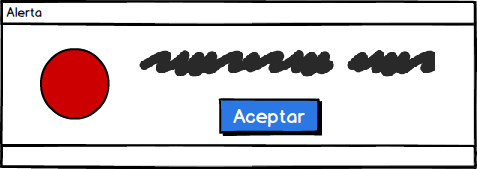
\includegraphics[width=0.5\textwidth]{./diseno/vescenarios/imagenes/alerta}
	\caption{Alerta Confirmación de Eliminación- Vista de Escenarios}
	\label{fig:Alerta4 - Vista de Escenarios}
\end{figure}
\subsection{CU7 Buscar Registro de Vehículo \label{sub:buscar registro}}
En este proceso no existe una pantalla como tal simplemente en la Visualización de la Agenda (figura \ref{fig:Pantalla Visualizar Agenda (busqueda)- Vista de Escenarios}) hay una barra de búsqueda en la parte superior donde el usuario podrá teclear el Número de Inventario del vehículo que desee. Si existe ese registro dentro de la base de datos, el sistema lo mostrará en la tabla. Caso contrario, si no existe, mostrará la tabla vacía. 
\begin{figure}[!h]
	\centering
	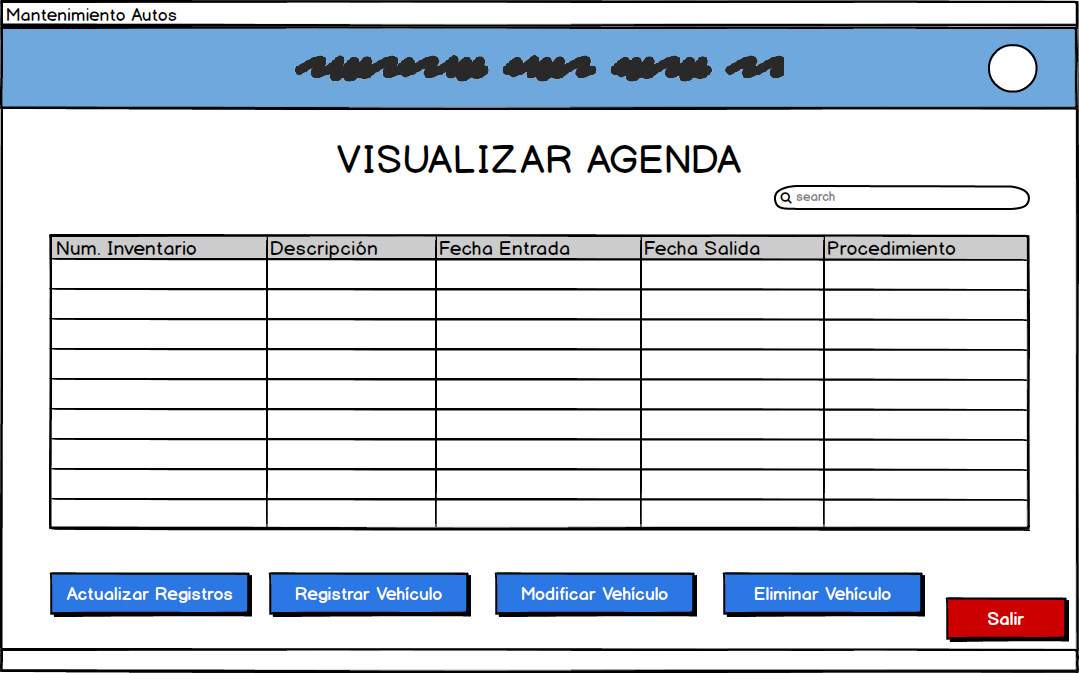
\includegraphics[width=1\textwidth]{./diseno/vescenarios/imagenes/VisualizarAgenda}
	\caption{Pantalla Visualizar Agenda (Búsqueda) - Vista de Escenarios}
	\label{fig:Pantalla Visualizar Agenda (busqueda)- Vista de Escenarios}
\end{figure}
\clearpage
\subsection{CU8 Visualizar Refacciones Disponibles}
Regresando un poco a la pantalla de Visualización del Menú (figura \ref{fig:Pantalla Visualizar Menu - Vista de Escenarios}), al pulsar el botón de 'Gestionar las Refacciones', aparece esta pantalla. Muy simular a la visualización de los registros pero aquí el usuario solamente podrá ver y buscar las refacciones que hay en existencia en el almacén del taller. En caso de que no exista alguno, podrá presionar el botón de la parte inferior 'Solicitar Refacción'.
\\
En la tabla el usuario podrá observar los registros a manera de lista dentro de una tabla, con los campos: Num. de Solicitud, una Descripción, la Fecha de Solicitud y la Existencia en almacén. 
\\
Al presionar el botón de salir, el sistema cerrará esta pantalla y regresará a la Visualización del Menú. 
\begin{figure}[!h]
	\centering
	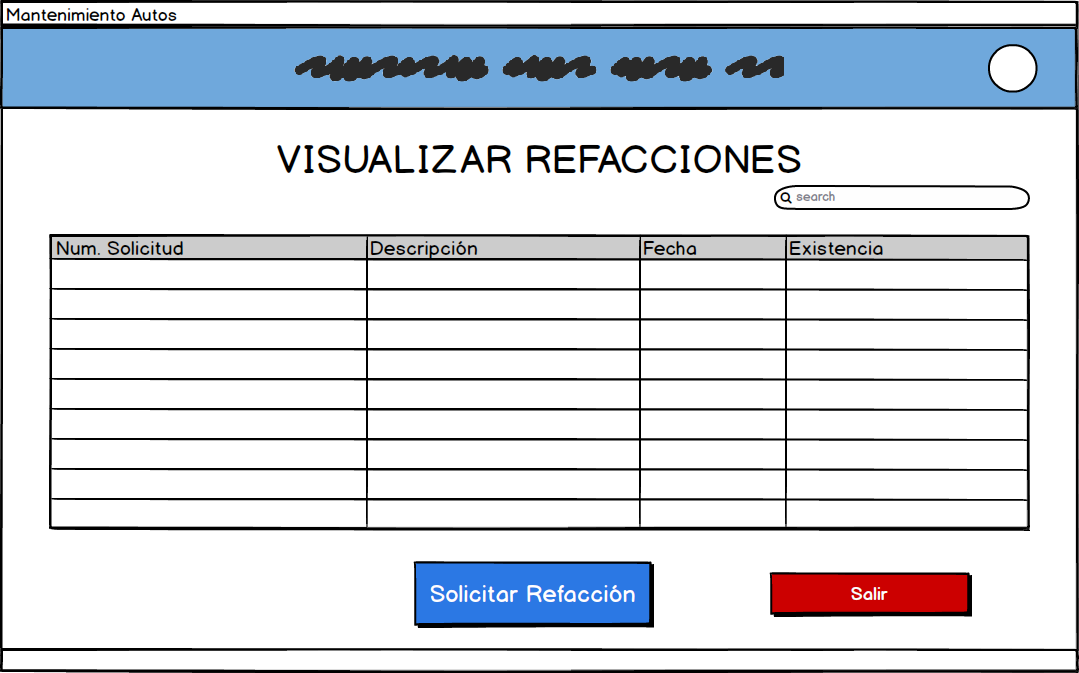
\includegraphics[width=1\textwidth]{./diseno/vescenarios/imagenes/VisualizarRefacciones}
	\caption{Pantalla Visualizar Refacciones - Vista de Escenarios}
	\label{fig:Pantalla Visualizar Refaccioes - Vista de Escenarios}
\end{figure}
\clearpage
\subsection{CU9 Solicitar Refacción}
Al entrar a esta parte del sistema, se despliega esta pantalla. Es un formulario de registro para la solicitud de alguna pieza en especifico. Solicitará un identificador (en este caso manejamos un Número de Solicitud), la Fecha en que se solicita y una Descripción donde se podrá agregar alguna otra información como el nombre o modelo. 
\\
Un vez llenado el formulario el usuario podrá pulsar el botón de 'Solicitar' para registrar esto en la base de datos. En caso de que el usuario desee salir de esta pantalla, simplemente deberá pulsar el botón 'Cancelar'.
\begin{figure}[!h]
	\centering
	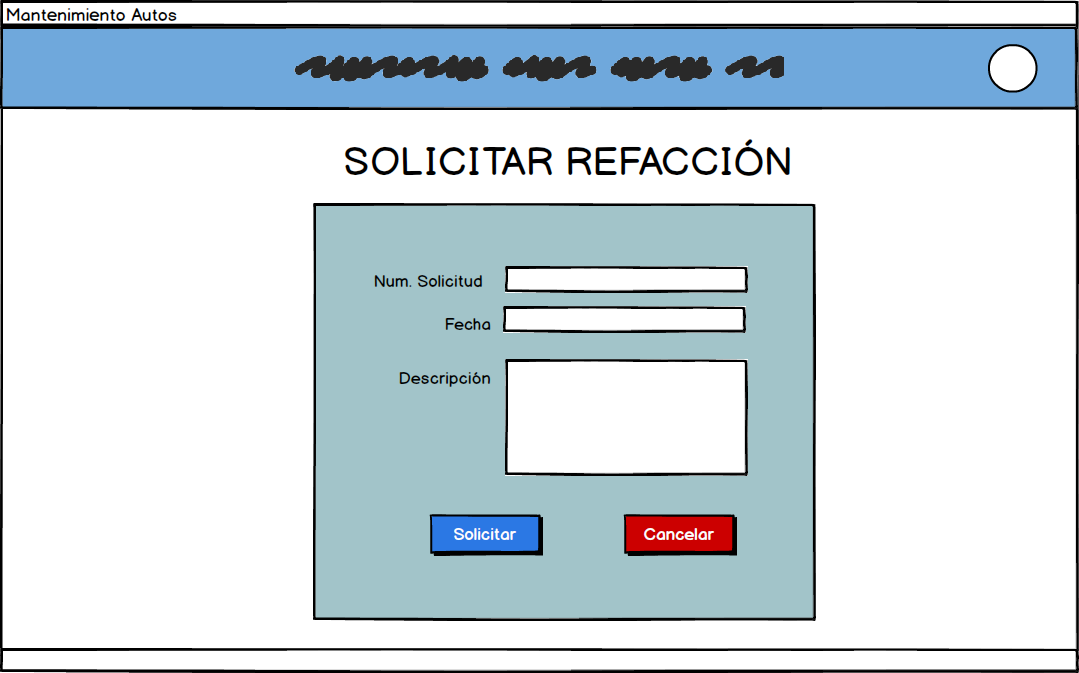
\includegraphics[width=1\textwidth]{./diseno/vescenarios/imagenes/solicitarRefaccion}
	\caption{Pantalla Solicitar Refacción - Vista de Escenarios}
	\label{fig:Pantalla Solicitar Refaccion - Vista de Escenarios}
\end{figure}
En caso de que el usuario ingrese de manera incorrecta alguno de los campos, el sistema mostrará un 'mensaje de alerta' (figura \ref{fig:Alerta5 - Vista de Escenarios}) informado del error que ha cometido. 
\begin{figure}[!h]
	\centering
	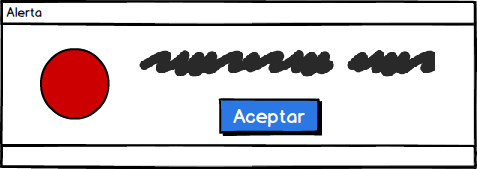
\includegraphics[width=0.4\textwidth]{./diseno/vescenarios/imagenes/alerta}
	\caption{Alerta Confirmación de Registro - Vista de Escenarios}
	\label{fig:Alerta5 - Vista de Escenarios}
\end{figure}
\subsection{CU10 Visualizar Empleados}
Cuando el administrador selecciona la opción 'Gestionar Empleados' del menú (figura \ref{fig:Pantalla Visualizar Menu Administrador - Vista de Escenarios}) aparece en pantalla la siguiente ventana. En ella se podrán visualizar a todos los empleados que están registrados dentro de la base de datos y que, obviamente, están trabajando dentro del taller. En la parte inferior de la ventana, existen más botones.
\begin{itemize}
	\item \textbf{Actualizar Registros:} Cuando se haga una acción en alguno de los registros, es necesario presionar este botón para que se actualicen todos los datos de la tabla-
	\item \textbf{Registrar Empleado:} Cuando se presiona este botón aparece una nueva ventana donde se podrá ingresar los datos de un nuevo empleado.
	\item \textbf{Modificar Empleado:} Al seleccionar una fila de la tabla (a un empleado registrado), aparecerá una ventana con un formulario de actualización.
	\item \textbf{Eliminar Empleado:} Al seleccionar una fila de la tabla (empleado registrado), aparecerá una ventana con un mensaje de seguridad para verificar si realmente se desea eliminar ese registro.
	\item \textbf{Salir:} El administrador cierra esa ventana y al mismo tiempo regresa al menú, figura \ref{fig:Pantalla Visualizar Menu Administrador - Vista de Escenarios}.
\end{itemize}
\begin{figure}[!h]
	\centering
	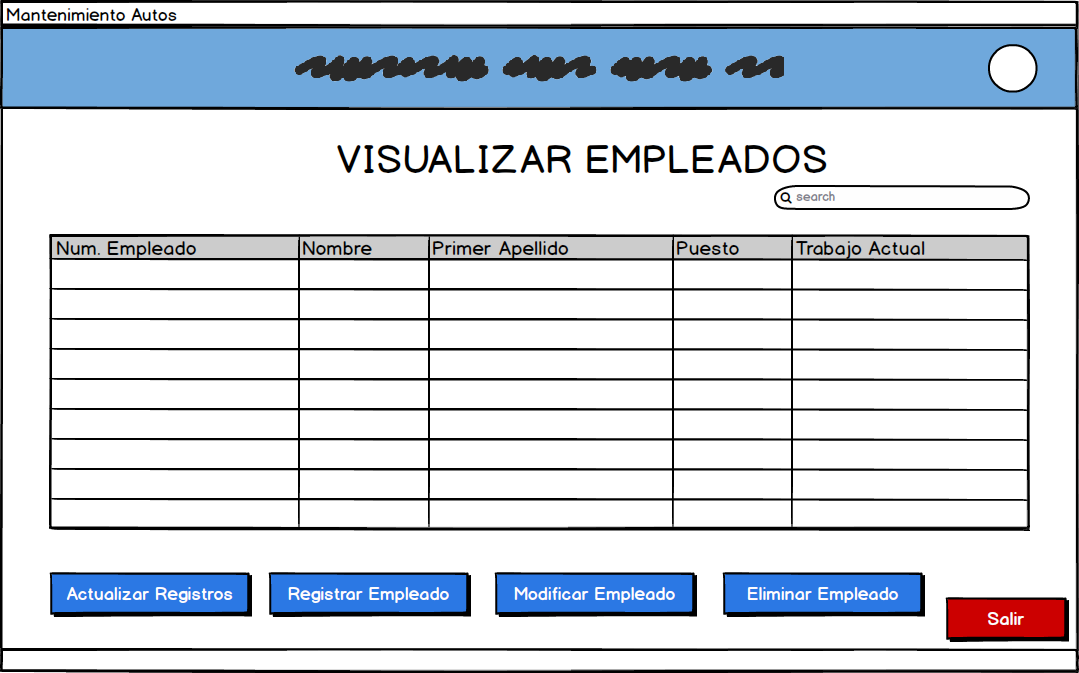
\includegraphics[width=1\textwidth]{./diseno/vescenarios/imagenes/VisualizarEmpleados}
	\caption{Pantalla Visualizar Empleados - Vista de Escenarios}
	\label{fig:Pantalla Visualizar Empleados - Vista de Escenarios}
\end{figure}
En dado caso de que se quiera modificar o eliminar un registro y no se ha seleccionado un renglón de la tabla, aparecerá un mensaje de alerta que le dirá al administrador que debe de seleccionar un registro.
\begin{figure}[!h]
	\centering
	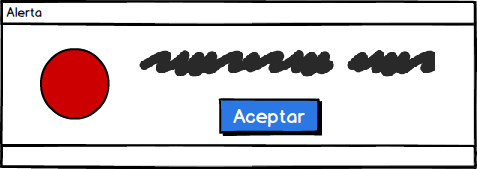
\includegraphics[width=0.5\textwidth]{./diseno/vescenarios/imagenes/alerta}
	\caption{Alerta - Vista de Escenarios}
	\label{fig:Alerta Empleados - Vista de Escenarios}
\end{figure}
\clearpage
\subsection{CU 11 Registrar Empleado}
En la siguiente ventana, figura \ref{fig:Pantalla Registrar Empleado - Vista de Escenarios}, se muestra un formulario de registro para un nuevo empleado donde el administrador podrá ingresar la información que el sistema le solicita para llevar a cabo el registro. Los datos que pide son: número de empleado (este será el usuario de cuenta del empleado), nombre completo y una contraseña que se le proporcionará al empleado una vez que el registro se haya hecho. En la parte inferior de la ventana, tenemos dos botones:
\begin{itemize}
	\item \textbf{Registrar:} Una vez llenados los campos, al dar click en este botón el sistema los validará y verificará si todos están llenos y con el formato adecuado, de no ser así se mostrará un mensaje de error (figura \ref{fig:Alerta Registro Empleados - Vista de Escenarios}) y el administrador debe de corregir el error de captura.
	\item \textbf{Cancelar: } El administrador desea salir de esa ventana, y el sistema regresa al a ventana 'Visualizar Empleados' (figura \ref{fig:Pantalla Visualizar Empleados - Vista de Escenarios}).
\end{itemize}
\begin{figure}[!h]
	\centering
	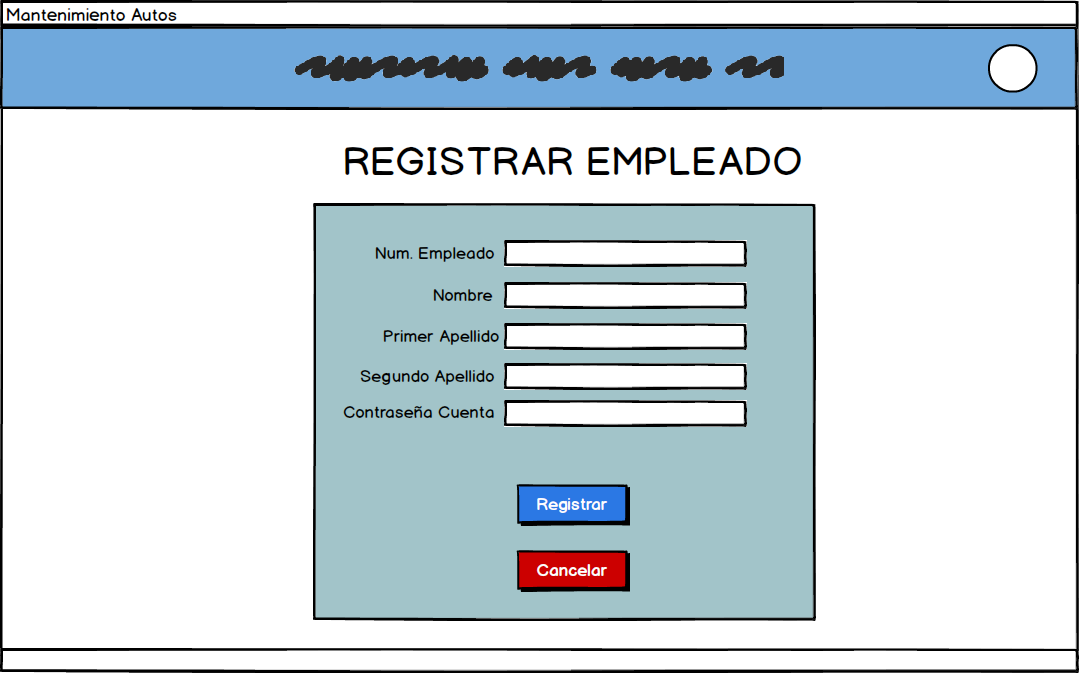
\includegraphics[width=0.8\textwidth]{./diseno/vescenarios/imagenes/registrarEmpleado}
	\caption{Pantalla Registrar Empleado - Vista de Escenarios}
	\label{fig:Pantalla Registrar Empleado - Vista de Escenarios}
\end{figure}
\begin{figure}[!h]
	\centering
	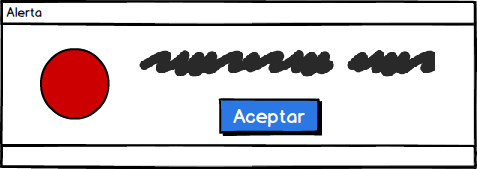
\includegraphics[width=0.3\textwidth]{./diseno/vescenarios/imagenes/alerta}
	\caption{Alerta Registro Empleados - Vista de Escenarios}
	\label{fig:Alerta Registro Empleados - Vista de Escenarios}
\end{figure}
\clearpage
\subsection{CU12 Modificar Empleado}
Al momento de seleccionar un registro de la pantalla de 'Visualizar Empleados' (figura \ref{fig:Pantalla Visualizar Empleados - Vista de Escenarios}) y seleccionar la opción de modificar el registro del empleado, se mostrará la ventana de modificación, la cual contiene un formulario de actualización de los datos. Cada uno de los campos estará lleno con la información que esta guardada dentro de la base de datos. El administrador podrá modificar dicha información y podrá seleccionar alguno de los botones de la parte inferior de la pantalla:
\begin{itemize}
	\item \textbf{Modificar:} Al dar click en esta opción, el sistema valida si toda la información es correcta (formato, estructura y si los campos están llenos). En caso de que no sea así, el sistema mostrará una alerta (figura \ref{fig:Alerta Modificar Empleado - Vista de Escenarios}).
	\item \textbf{Cancelar:} Salir de esa ventana y regresar a al pantalla anterior. (Figura \ref{fig:Pantalla Visualizar Empleados - Vista de Escenarios}).
\end{itemize}
\begin{figure}[!h]
	\centering
	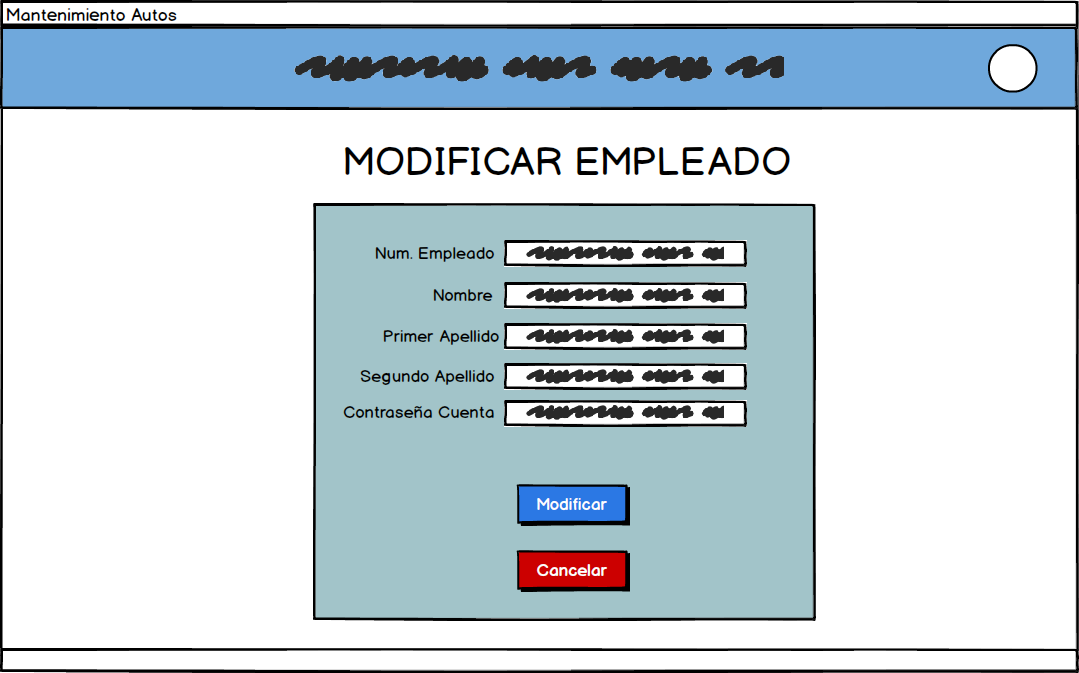
\includegraphics[width=0.8\textwidth]{./diseno/vescenarios/imagenes/modificarEmpleado}
	\caption{Pantalla Modificar Empleado - Vista de Escenarios}
	\label{fig:Pantalla Modificar Empleado - Vista de Escenarios}
\end{figure}
\begin{figure}[!h]
	\centering
	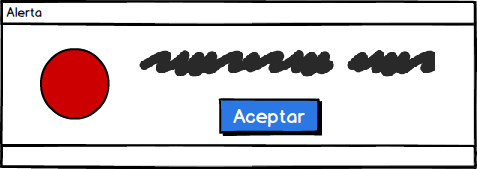
\includegraphics[width=0.3\textwidth]{./diseno/vescenarios/imagenes/alerta}
	\caption{Alerta Modificar Empleado - Vista de Escenarios}
	\label{fig:Alerta Modificar Empleado - Vista de Escenarios}
\end{figure}
\clearpage
\subsection{CU13 Eliminar Empleado}
Esta pantalla funciona como un mensaje de seguridad. Al seleccionar un registro de la pantalla 'Visualizar Empleado' y el administrador selecciona la opción de eliminar empleado, se mostrará la siguiente pantalla. Aqui se muestran los datos del empleado que se desea eliminar y dos opciones:
\begin{itemize}
	\item \textbf{Aceptar:} El sistema interactúa con la base de datos y se logra eliminar el registro del empleado. Una vez eliminado, el sistema mostrará un mensaje que el proceso a sido exitoso. (Figura \ref{fig:Alerta Eliminar Empleado - Vista de Escenarios}).
	\item \textbf{Cancelar:} 
\end{itemize}
\begin{figure}[!h]
	\centering
	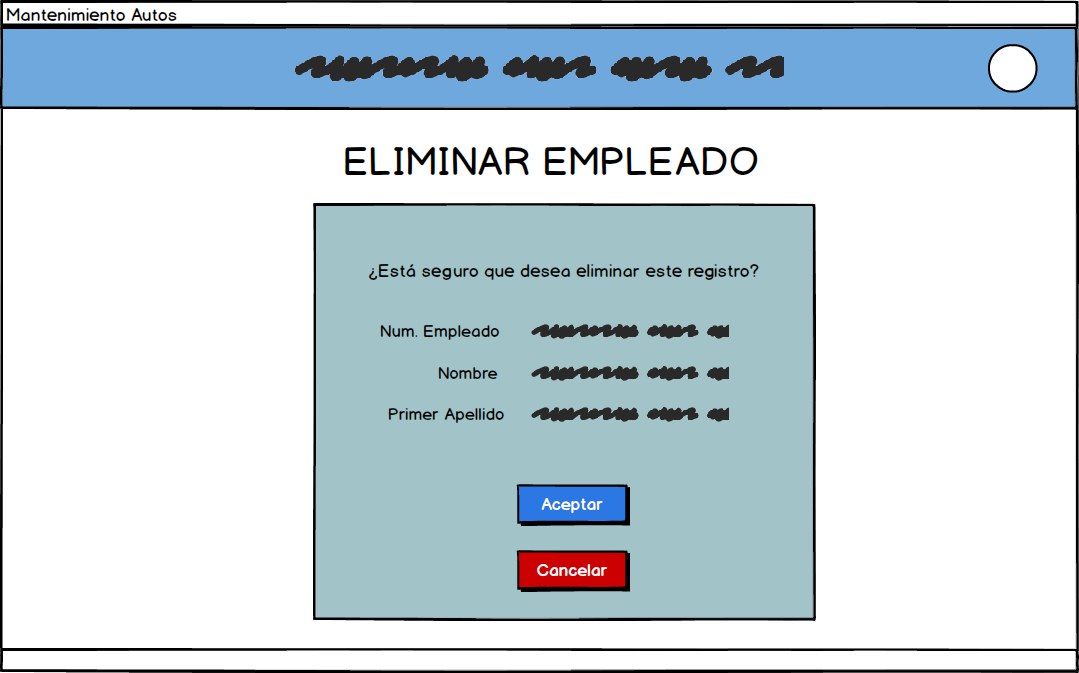
\includegraphics[width=0.8\textwidth]{./diseno/vescenarios/imagenes/eliminarEmpleado}
	\caption{Pantalla Eliminar Empleado - Vista de Escenarios}
	\label{fig:Pantalla Eliminar Empleado - Vista de Escenarios}
\end{figure}
\begin{figure}[!h]
	\centering
	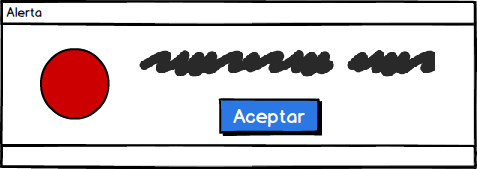
\includegraphics[width=0.5\textwidth]{./diseno/vescenarios/imagenes/alerta}
	\caption{Alerta Eliminar Empleado - Vista de Escenarios}
	\label{fig:Alerta Eliminar Empleado - Vista de Escenarios}
\end{figure}
\clearpage
\subsection{CU14 Buscar Empleado}
Para este proceso, el sistema no tiene destinado una pantalla completamente, solo es una pequeña barra de búsqueda en la parte superior derecha de la pantalla 'Visualizar Empleados' (figura \ref{fig:Pantalla Visualizar Empleado (Busqueda) - Vista de Escenarios}). En dicha barra, el administrador podrá ingresar el Número de Empleado que desee. Si existe el registro dentro de la base de datos, el sistema lo mostrara directamente en la tabla. Caso contrario, mostrará la tabla vacía.
\begin{figure}[!h]
	\centering
	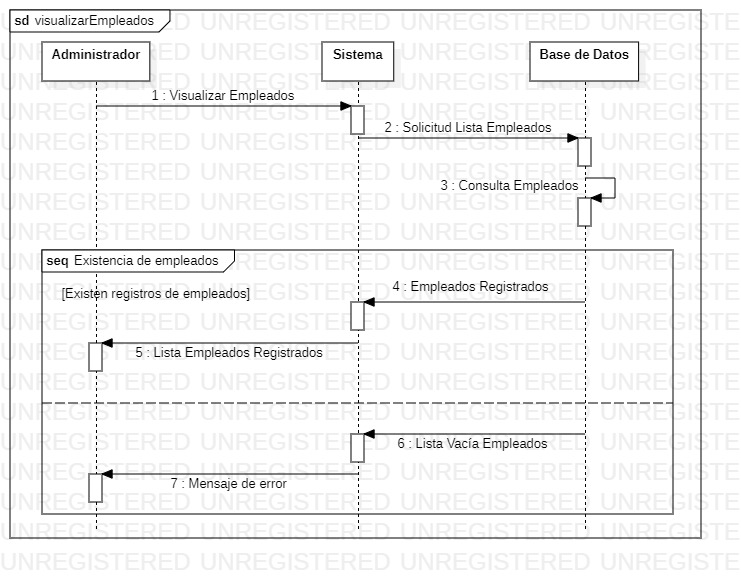
\includegraphics[width=1\textwidth]{./diseno/vescenarios/imagenes/visualizarEmpleados}
	\caption{Pantalla Visualizar Empleado (Búsqueda) - Vista de Escenarios}
	\label{fig:Pantalla Visualizar Empleado (Busqueda) - Vista de Escenarios}
\end{figure}
\clearpage
\subsection{CU15 Visualizar Refacciones}
En esta ventana, el administrador puede visualizar todas las refacciones que se encuentran dentro del almacén del taller. Esta tabla posee tres columnas, el Número de Inventario de la refacción, la descripción de la misma refacción y por último el vehículo para el que se necesita. En la parte inferior de la ventana tenemos varias opciones:
\begin{itemize}
	\item \textbf{Actualizar Registros:} Una vez que se haya realizado una acción con algún registro de la tabla, el administrador debe de dar click en este botón para que todas las filas y columnas de la tabla se actualicen.
	\item \textbf{Registrar Refacción:} Se despliega una pantalla donde el administrador podrá ingresar los datos necesarios para hacer un registro de una refacción.
	\item \textbf{Modificar Refacción:} En caso de que se necesite modificar por alguna razón un registro de refacción se podrá hacer con esta ocpción.
	\item \textbf{Eliminar Refacción:} Cuando se requiera eliminar un registro de una refacción por la razón que sea, esta opción ayudará al administrador a hacerlo desplegando un mensaje de seguridad.
	\item \textbf{Salir: }El sistema regresará a la ventana del menú del administrador, figura \ref{fig:Pantalla Visualizar Menu Administrador - Vista de Escenarios}. 
\end{itemize}
En caso de que no se seleccione una fila dentro de la tabla y se desee modificar o eliminar algún registro de la refacción se mostrará un mensaje de error y el administrador será enterado del error que está cometiendo. 
\begin{figure}[!h]
	\centering
	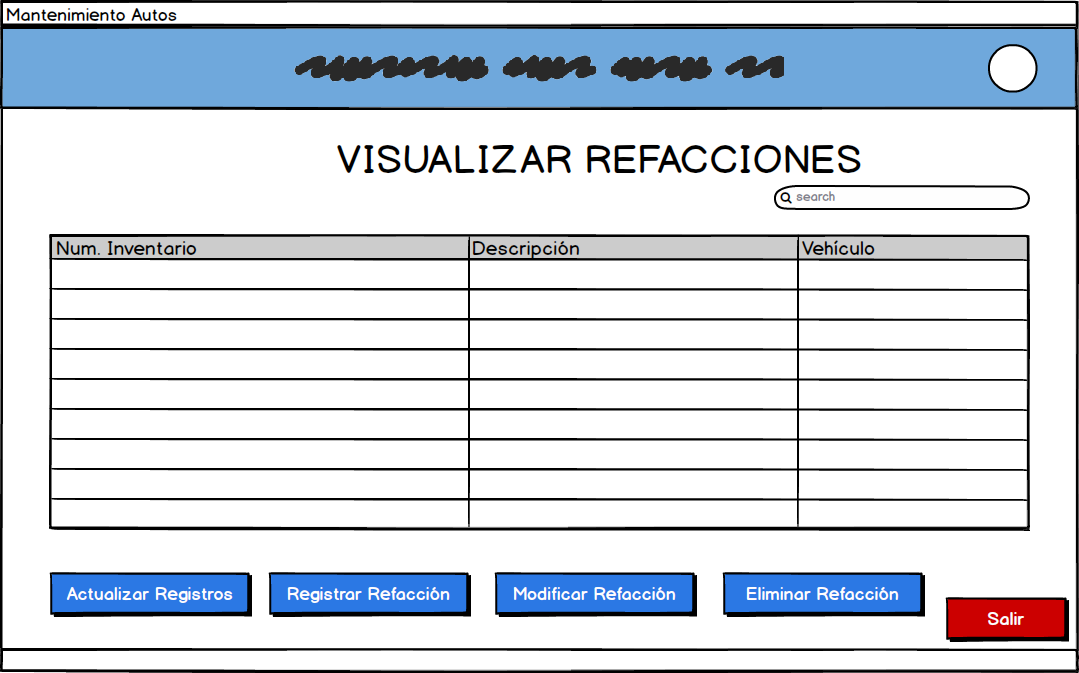
\includegraphics[width=1\textwidth]{./diseno/vescenarios/imagenes/VisualizasRefacciones}
	\caption{Pantalla Visualizar Refacciones Administrador - Vista de Escenarios}
	\label{fig:Pantalla Visualizar Refacciones Administrador - Vista de Escenarios}
\end{figure}
\begin{figure}[!h]
	\centering
	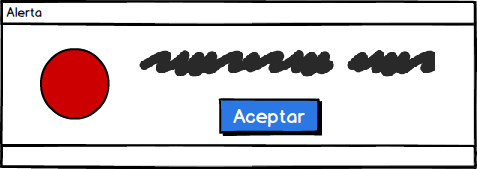
\includegraphics[width=0.5\textwidth]{./diseno/vescenarios/imagenes/alerta}
	\caption{Alerta Refacciones- Vista de Escenarios}
	\label{fig:Alerta Refacciones - Vista de Escenarios}
\end{figure}
\clearpage
\subsection{CU16 Registrar Refacción}
Esta pantalla aparece cuando el administrador elige la opción de registrar una refacción desde la pantalla de 'Visualizar Refacciones, (figura\ref{fig:Pantalla Visualizar Refacciones Administrador - Vista de Escenarios}). En esta sección, el sistema solicita que el administrador ingrese la información para hacer el registro eb este caso es el Número de Inventario, para que Vehículo va destinado y por último una descripción de la refacción que se va a utilizar. En la parte inferior de la pantalla, tenemos dos botones con diferentes opciones:
\begin{itemize}
	\item \textbf{Registrar:} Al dar click en este botón, el sistema validará cada uno de los campos que han sido llenados, su formato y su contenido. En caso de que exista un error, el propio sistema mostrará un mensaje de error para que el administador corrija el error.
	\item \textbf{Cancelar:} El sistema regresa a la pantalla anterior \ref{fig:Pantalla Visualizar Refacciones Administrador - Vista de Escenarios} sin hacer algún registro.
\end{itemize} 
\begin{figure}[!h]
	\centering
	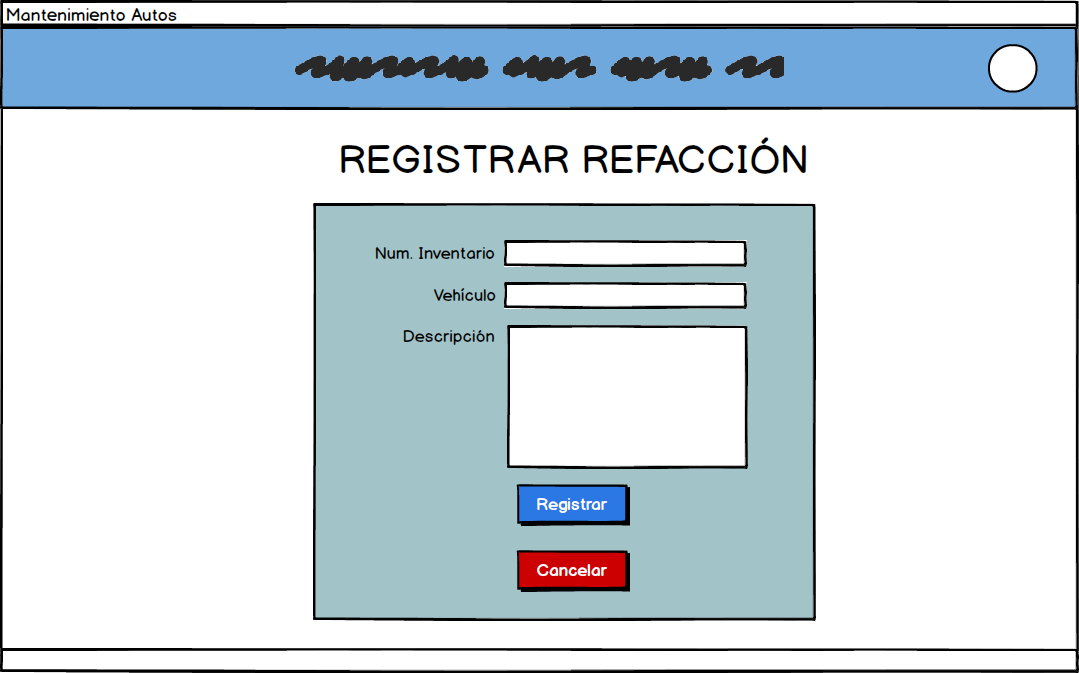
\includegraphics[width=0.8\textwidth]{./diseno/vescenarios/imagenes/registrarRefacciones}
	\caption{Pantalla Registrar Refacción - Vista de Escenarios}
	\label{fig:Pantalla Registrar Refacción - Vista de Escenarios}
\end{figure}
\begin{figure}[!h]
	\centering
	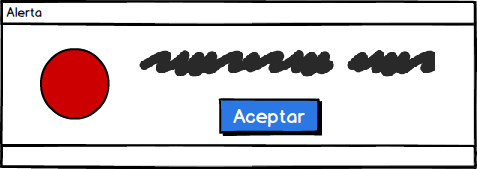
\includegraphics[width=0.3\textwidth]{./diseno/vescenarios/imagenes/alerta}
	\caption{Alerta Registro Refacciones- Vista de Escenarios}
	\label{fig:Alerta Registro Refacciones - Vista de Escenarios}
\end{figure}
\subsection{CU17 Modificar Refacción}
Cuando el administrador elige la opción de modificar un registro, se despliega esta pantalla donde el sistema muestra un formulario de actualización donde todos los campos están llenos con la información que está dentro de la base de datos. En la parte inferior de esta ventana tenemos dos botones:
\begin{itemize}
	\item \textbf{Modificar:} Al dar click en este botón, el sistema validará nuevamente todos los campos hayan sido modificados o no, validando si están llenos y su formato. 
	\item \textbf{Cancelar:} El sistema regresa a la pantalla anterior (figura \ref{fig:Pantalla Visualizar Refacciones Administrador - Vista de Escenarios}) sin modificar ningún dato. 
\end{itemize}
\begin{figure}[!h]
	\centering
	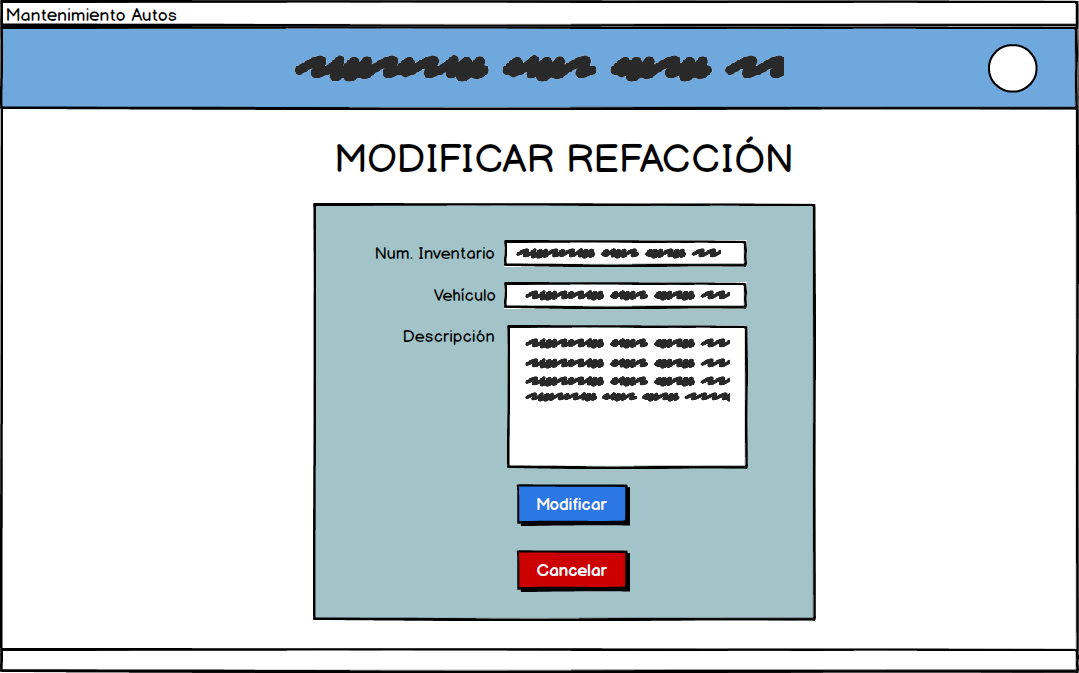
\includegraphics[width=0.8\textwidth]{./diseno/vescenarios/imagenes/modificarRefaccion}
	\caption{Pantalla Modificar Refacciones  - Vista de Escenarios}
	\label{fig:Pantalla Modificar Refacción - Vista de Escenarios}
\end{figure}
\begin{figure}[!h]
	\centering
	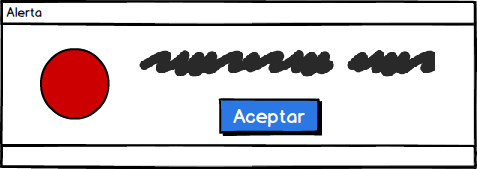
\includegraphics[width=0.3\textwidth]{./diseno/vescenarios/imagenes/alerta}
	\caption{Alerta Modificar Refacciones- Vista de Escenarios}
	\label{fig:Alerta Registro Refacciones - Vista de Escenarios}
\end{figure}
\clearpage
\subsection{CU18 Eliminar Refacción}
Esta pantalla funciona como un mensaje de seguridad, este se asegurará que el administrador realmente quiere eliminar el registro que ha seleccionado de una refacción, mostrará toda la información que se tiene sobre esa refacción. En la parte inferior hay dos botones:
\begin{itemize}
	\item \textbf{Aceptar:} El sistema elimina el registro seleccionado por el administrador y muestra un mensaje de confirmación que el proceso ha sido exitoso.
	\item \textbf{Cancelar:} El sistema regresa a la pantalla anterior (figura \ref{fig:Pantalla Visualizar Refacciones Administrador - Vista de Escenarios}) sin hacer alguna modificación.
\end{itemize}
{\begin{figure}[!h]
	\centering
	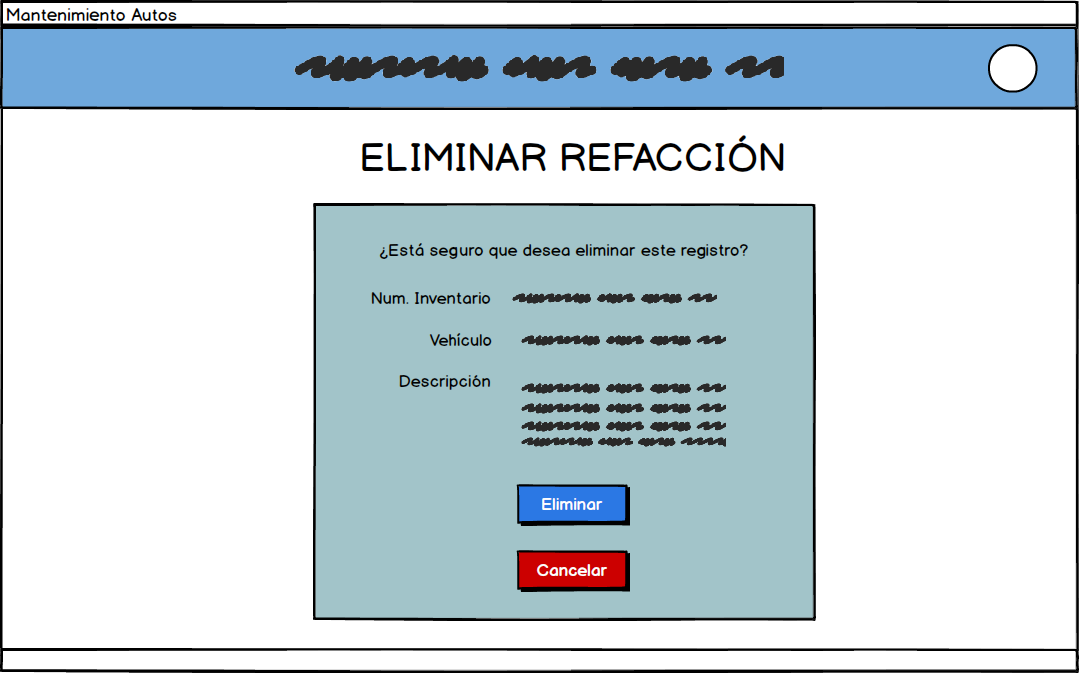
\includegraphics[width=0.8\textwidth]{./diseno/vescenarios/imagenes/eliminarRefaccion}
	\caption{Pantalla Eliminar Refacciones  - Vista de Escenarios}
	\label{fig:Pantalla Eliminar Refacción - Vista de Escenarios}
\end{figure}
\begin{figure}[!h]
	\centering
	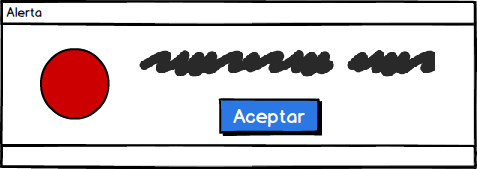
\includegraphics[width=0.3\textwidth]{./diseno/vescenarios/imagenes/alerta}
	\caption{Alerta Eliminar Refacciones- Vista de Escenarios}
	\label{fig:Alerta Eliminar Refacciones - Vista de Escenarios}
\end{figure}
\clearpage
\subsection{CU19 Buscar Refacciones}
Para la búsqueda de una refacción el sistema no tiene un módulo destinado como tal, es simplemente una barra de búsqueda en la parte superior derecha donde el administrador podrá ingresar el número de inventario de alguna refacción, en caso de que exista se mostrará la información en la tabla si no es así, la tabla se mostrará vacía. 
\begin{figure}[!h]
	\centering
	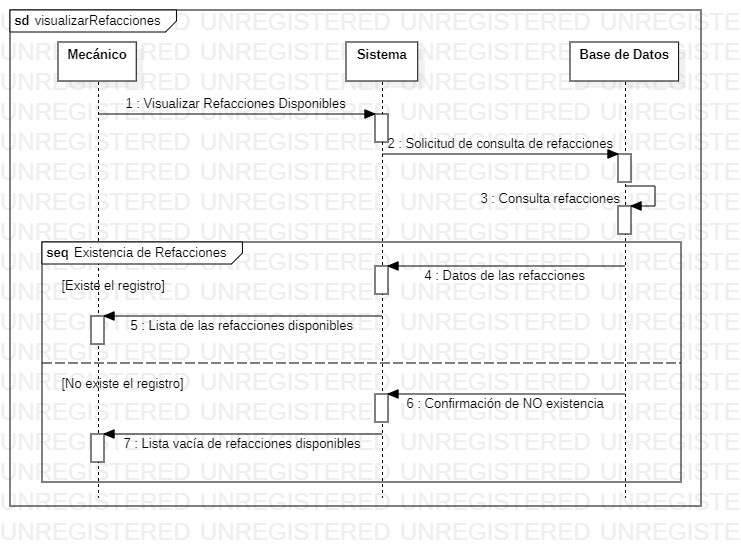
\includegraphics[width=0.8\textwidth]{./diseno/vescenarios/imagenes/visualizarRefacciones}
	\caption{Pantalla Visualizar Refacciones Admin (Búsqueda) - Vista de Escenarios}
	\label{fig:Pantalla refacciones busqueda- Vista de Escenarios}
\end{figure}
\clearpage
\subsection{CU20 Visualizar Solicitudes}
En esta pantalla, el administrador podrá visualizar en una tabla cada una de las solicitudes de refacción que los empleados han hecho. Esta tabla consta de tres columnas, la primera es el número de Inventario de la refacción, la segunda es el nombre del empleado que solicitó la refacción y la tercera es una descripción de la refacción. Solo consta de tres opciones en la parte inferior de la ventana:
\begin{itemize}
	
	\item \textbf{Atender Solicitud:} En esta opción se desplegará una pantalla donde el administrador podrá verificar la solicitud y aceptarla. En caso de que no se elija una fila de la tabla, se mostrará un mensaje de error en pantalla. (Figura \ref{fig:Alerta Solicitudes - Vista de Escenarios}).
	\item \textbf{Salir:} Regresará a la pantalla anterior la cual es el Menú del administrador (figura \ref{fig:Pantalla Visualizar Menu Administrador - Vista de Escenarios}).
\end{itemize}
\begin{figure}[!h]
	\centering
	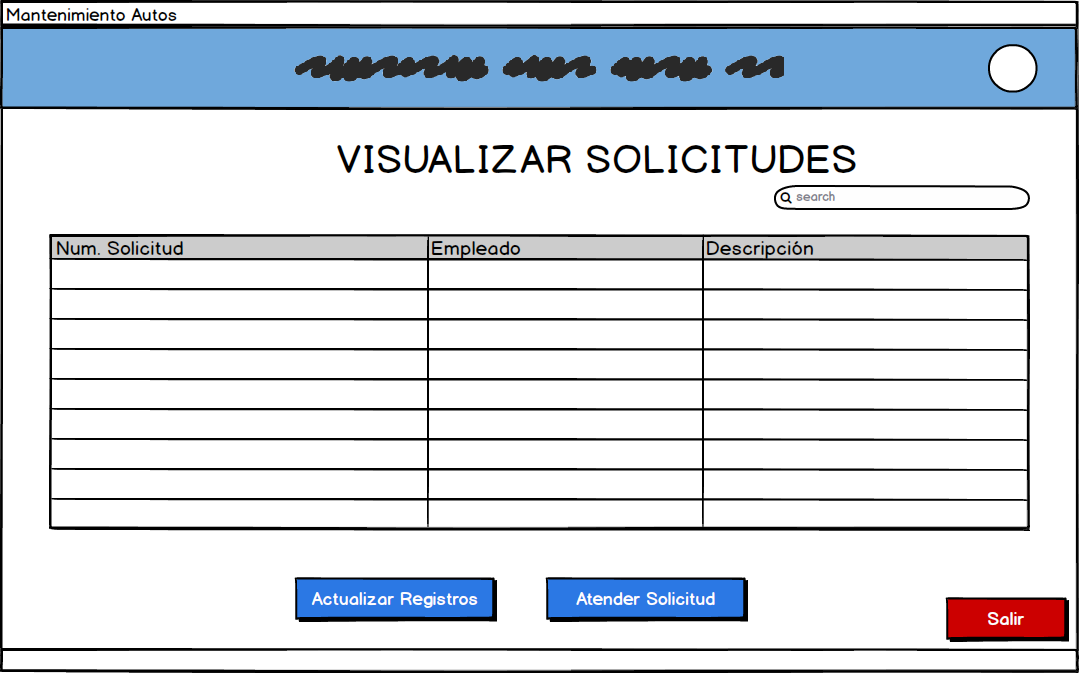
\includegraphics[width=0.8\textwidth]{./diseno/vescenarios/imagenes/visualizarSolicitudes}
	\caption{Pantalla Visualizar Solicitudes - Vista de Escenarios}
	\label{fig:Pantalla Visualizar Solicitudes- Vista de Escenarios}
\end{figure}
\begin{figure}[!h]
	\centering
	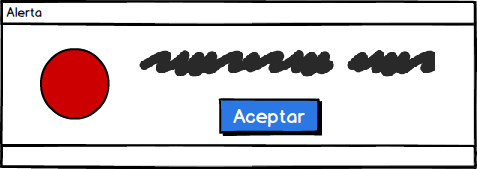
\includegraphics[width=0.3\textwidth]{./diseno/vescenarios/imagenes/alerta}
	\caption{Alerta Solicitudes- Vista de Escenarios}
	\label{fig:Alerta Solicitudes - Vista de Escenarios}
\end{figure}
\clearpage
\subsection{CU21 Atender Solicitud}
Esta pantalla mostrará todos los datos de la solicitud que se haya seleccionado, aquí el administrador podrá aprobar la solicitud una vez que el proveedor haya conseguido la refacción que se necesita. El botón de cancelar regresa a la pantalla anterior de visualizar solicitudes (figura \ref{fig:Pantalla Visualizar Solicitudes- Vista de Escenarios}) y el administrador podrá seguir interactuando con el sistema. 
\begin{figure}[!h]
	\centering
	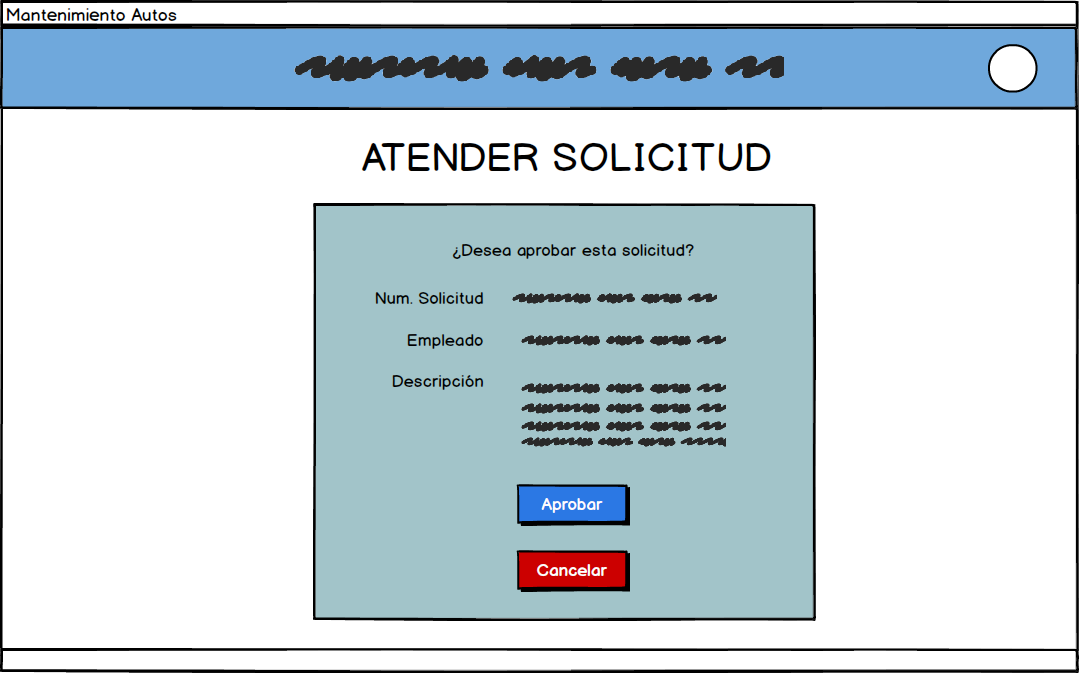
\includegraphics[width=0.8\textwidth]{./diseno/vescenarios/imagenes/eliminarSolicitud}
	\caption{Pantalla Atender Solicitud - Vista de Escenarios}
	\label{fig:Pantalla Atender - Vista de Escenarios}
\end{figure}
\clearpage